\section{Formal: Assignment 2}
\textbf{Contribution of Laodice Melliti:} Implementation scope, algorithmic design and description, implemented system architecture graphic\\
\textbf{Contribution of Jonas Helbig:}  Implementation scope, algorithmic design and description\\
\section{Implementation scope}
The system as presented by us so far is too comprehensive to be fully implemented during this project. We this section we will give an estimation about which parts of the system can actually be implemented by us in the scope of this project.

Instead of focusing on emergency response systems with functions like detecting heart attacks, sleep attacks or even death during driving, we implement a system for long term measurement and monitoring of the user.
We focus on three different health values, namely the heart beat, the breathing rate and the blood pressure. Our system is intended to be used by elderly people or people with illnesses affecting one of those parameters. 
We create a system capable of detecting unusual or undesirable development of a persons health over a longer period of 30-100 days.

In short, our system will create long term trends on the development of the user's health status. While doing that it is smart enough to detect unusal values and assess them in cooperation with the user to reduce or increase their influence on the trend.
The process is further described in listing
\begin{enumerate}
	\item For the initial setup of the training, we recommend the visit of a doctor. Since every patient has a different medical history, a doctor has to determine through several appropriate test the ``normal'' condition of the patient in reference to our desired parameters. After the initial setup, the system will be activated every time the users uses his car.
	\item During each session the system will capture the parameters from the user, prepare and normalize the data and extract the features
	\item The extracted features (as described later) will be processes by our system with the algorithms described in the next section
	\item The system will react to unusual values, outside of the boundary predetermined by a doctor in the first step and it will try to find reasonable explanations in cooperation with the user, with a predefined question catalog. The questions can be answered binary, so that the user could easily give feedback without being distracted while driving 
	\item Depending on the responds of the user, the system will adjust its validation and weighting system for the calculation of the long term rating
	\item Those ratings determined over a longer time will be repeatedly presented to the user, together with recommendations on how to react 
\end{enumerate}

To reduce the complexity and avoid handling raw medical data, we are only implementing the steps three to six. The other steps would be scope of another research paper and should focus on the practicality of the extraction of the desired data.
From the different sensors and actuators described in the last section we are going to use the following ones:
\begin{itemize}
	\item Hear belt: From this sensor we use the heart beat rate and the breathing rate which is continuously measured. For our purpose, we assume that we get the values as heart beat per second.
	\item Blood pressure meter: From this sensor we use both the systolic and the diastolic blood pressure values. For our purpose, we assume that we get the values as millimeters of mercury
	\item GPS: For each dataset we save in the database we save the approximate GPS location
\end{itemize}
The process is summarized in figure \ref{fig:flow}.
\begin{figure}
	\graphitemize{Phase 1,Phase 2, Phase 3, Phase 4, Phase 5, Phase 6}
	\caption{Process flow of our implementation}
	\label{fig:flow}
\end{figure}

\section{Algorithmic approach}
The pseudo code for our approach is specified through the algorithms \ref{alg:capture} and \ref{alg:longterm}.
We focus on the important functions and aspects, without going into details about the capturing and preparation of the data.
All the important functions and variables used are described below.
\begin{algorithm}[htbp]
	\begin{algorithmic}[1]
		\Require{None}
		\Ensure{Database, Session trend}
		\Repeat
		\State $data \gets$ \Call{CaptureData()}{}
		\State $data \gets$ \Call{PrepareData}{$data$}
		\State $data \gets$ \Call{ExtractFeatures()}{} \Comment{data: concrete numbers of BP/ BR and HB?}
		\State $median \gets$ \Call{Average}{$data$} \Comment{Average of the last 5 minutes}
		\State $weight \gets 1$ 
		\State $GPScoordinates \gets$ \Call{GetGPS()}{}
		\State $weight \gets 1$  \Comment{Default value for the weighting function}
		\If {\Call{OutsideBoundaries}{$median$}}
			\State $response \gets$ \Call{AskUserQuestions()}{}
			\If {$response == yes$} \Comment{yes: valid reason for data out of boundaries}
				\State \Call{ReduceWeight()}{}
			\Else
				\State \Call{IncreaseWeight()}{}			\EndIf
		\EndIf
				
		\State \Call{Store}{$median$, $weight$, $GPScooridinates$} \Comment{Save values in Database}
		\Until{Driving session is over}
		\State \Call{SessionEvaluation()}{}	\Comment{Presented at the end of each driving session}
	\end{algorithmic}
	\caption{Capturing, processing and storing the data}
	\label{alg:capture}
\end{algorithm}
		%%%%%%%%
\begin{algorithm}[htbp]
	\begin{algorithmic}[1]	
		\Require Database
		\Ensure Recommendation for the user
		\Repeat
		\State $data \gets$ \Call{ReadDatabase()}{}
		\State $rating \gets 0$	
		\ForAll {$dataset$ in $data$} \Comment{every dataset consists of median, weight and gps}
		\State $rating \gets rating + weight * median$
		\EndFor
		\State $rating \gets rating  data.lenght$ \Comment{Average with weight}
		\If {\Call{OutsideBoundaries}{$rating$}}
			\State \Call{makeRecommendation()}{}
		\EndIf
		\Until{24 hours are over}
	\end{algorithmic}
	\caption{Long term monitoring}
	\label{alg:longterm}
\end{algorithm}

\paragraph{Detailed explanation for Algorithm \ref{alg:capture}}
\begin{description}
	\item [CaptureData()] For the heart beat and breath rate : we capture the data every seconds. For the blood pressure, we capture the data every 30 minutes
	\item [PrepareData(data)] We normalyse the data received and reduce the noise as much as possible.
	\item [ExtractFeatures()] The data we previously captured is analog and we need digital data for the analysis. As such, we convert the analog data into digital data.
	\item [Average()] Every 5 minutes, we make a average of all the data received.
	\item [GetGPS()] Get the current GPS position
	\item [OutsideBoundaries(median)] We check if the data is outside the boundaries. Those boundaries are set up by a doctor when the system is implemented in the car. This function return a boolean variable\\
	True : the data is outside the boundaries\\
	False : the data is inside the boundaries. In this case we assume everything is fine
	\item [AskUserQuestion()] We ask the driver if he had exerciced recently and if he is feeling unwell or stressed. If the answer to any of this questions is yes, then the function return a boolean variable set to true. Otherwise, it returns false.
\item [Store(median, weight, GPScooordinates)] We store together all the medians, their weight and the GPS coordinates assiociated into the database.
\item [SessionEvaluation()] We make an average of all the data received dureing the drivinig session so that we can compare two driving session one to the other.
\end{description}
\paragraph{Detailed explanation for Algorithm \ref{alg:longterm}}
\begin{description}
	\item [ReadDatabase()] We put a specific anount of data into a new variable to analyse this whithout accidently changing our saved data.
	\item [OutsideBoundaries()] See function capture
	\item [MakeRecommendation()] Depending of the result, we either make recommendation to see a Doctor (via speakers) or we inform the driver that everything is fine.
\end{description}

\newpage
\section{Updated system architecture}
\begin{figure}[h]
	\centering
	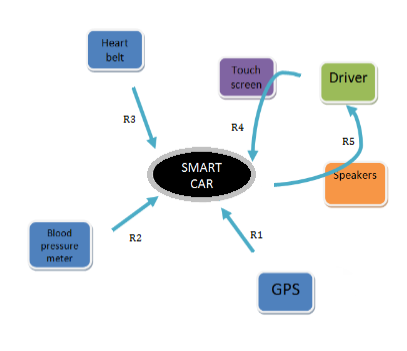
\includegraphics[scale=0.8]{./images/implementationArchitecture}		%Include picture
	\caption{System Architecture redefined for the scope of our project}					%Picture caption
	\label{fig:impsys}									%Label of the picture, can be referenced with \ref{fig:impsys}
\end{figure}

\begin{description}\addtolength{\itemsep}{-0.5\baselineskip}
	\item{R1:} Get the GPS position
	\item{R2:} Get the extracted features for the blood pressure
	\item{R3:} Get the extracted features for the breathing rate and the heart beat
	\item{R4:} Receive response from user
	\item{R5:} Ask user questions

	
	If needed, it uses the GPS coordinates (sensor).
\end{description}